%=========================================================
% Mathematics Report Template - HD Standard
%=========================================================
\documentclass[11pt,a4paper]{article}

%---------------- Packages ----------------
\usepackage[utf8]{inputenc}
\usepackage[T1]{fontenc}
\usepackage{lmodern}
\usepackage{geometry}
\usepackage{multicol}
\geometry{a4paper, margin=2.5cm}
\usepackage{tikz}
\usetikzlibrary{calc}
\usetikzlibrary{angles,quotes} % for angle marks
\usepackage{tabularx}
\usepackage{booktabs}
\usepackage{multirow}
\usetikzlibrary{arrows.meta, positioning}
\usepackage{float}
\usepackage{setspace}
\usepackage[skip=0.6\baselineskip, indent=0pt]{parskip} % no paragraph indent, vertical gap instead
\usepackage{algorithm}
\usepackage{algpseudocode}
% optional: make comments right-aligned with a pointer
\algrenewcommand\algorithmiccomment[1]{\hfill$\triangleright$~#1}

\usepackage{amsmath, amssymb, amsthm, mathtools} % math environments
\usepackage{mathrsfs}
\usepackage{bm}             % bold math symbols
\usepackage{physics}        % derivatives, bra-ket, etc.
\usepackage{enumitem}       % custom lists
\usepackage{tikz}           % diagrams
\usepackage{pgfplots}       % plots
\pgfplotsset{compat=1.18}
\usepackage{graphicx}       % figures
\usepackage{subcaption}     % subfigures
\usepackage{xcolor}         % colors
\usepackage{hyperref}       % hyperlinks
\hypersetup{colorlinks=true, linkcolor=black, citecolor=blue, urlcolor=blue}

%---------------- Theorem Environments ----------------
\newtheorem{theorem}{Theorem}[section]
\newtheorem{lemma}[theorem]{Lemma}
\newtheorem{proposition}[theorem]{Proposition}
\newtheorem{corollary}[theorem]{Corollary}
\theoremstyle{definition}
\newtheorem{definition}[theorem]{Definition}
\newtheorem{example}[theorem]{Example}
\theoremstyle{remark}
\newtheorem{remark}[theorem]{Remark}


% ---- colours and shorthands for the expansion factors ----
\definecolor{x3dgreen}{RGB}{0,150,90}
\definecolor{x3dblue}{RGB}{60,60,205}
\definecolor{x3dviolet}{RGB}{140,60,200}
\definecolor{x3dmagenta}{RGB}{190,20,140}
\definecolor{x3dbrown}{RGB}{150,60,10}
\newcommand{\xgtau}{\textcolor{x3dgreen}{\bm{\gamma_\tau}}}
\newcommand{\xgt}{\textcolor{x3dgreen}{\bm{\gamma_t}}}
\newcommand{\xgs}{\textcolor{x3dblue}{\bm{\gamma_s}}}
\newcommand{\xgw}{\textcolor{x3dviolet}{\bm{\gamma_w}}}
\newcommand{\xgb}{\textcolor{x3dmagenta}{\bm{\gamma_b}}}
\newcommand{\xgd}{\textcolor{x3dbrown}{\bm{\gamma_d}}}
% one shaded cuboid: #1 x, #2 y, #3 width (C), #4 height (H,W), #5 depth (T)
\newcommand{\xslab}[5]{%
    \pgfmathsetmacro{\slabdx}{0.55*#5}%
    \pgfmathsetmacro{\slabdy}{0.42*#5}%
    \shadedraw[line width=0.25pt, left color=orange!45, right color=black!40]
        (#1,#2+#4) -- (#1+#3,#2+#4) -- (#1+#3+\slabdx,#2+#4+\slabdy) -- (#1+\slabdx,#2+#4+\slabdy) -- cycle;
    \shadedraw[line width=0.25pt, top color=black!45, bottom color=orange!35]
        (#1+#3,#2) -- (#1+#3,#2+#4) -- (#1+#3+\slabdx,#2+#4+\slabdy) -- (#1+#3+\slabdx,#2+\slabdy) -- cycle;
    \shadedraw[line width=0.25pt, inner color=black!22, outer color=orange!45]
        (#1,#2) rectangle (#1+#3,#2+#4);
}
% a res stage: three slabs side by side. #1 x, #2 y, #3 slab width, #4 height, #5 depth, #6 gap
\newcommand{\xstage}[6]{%
    \foreach \i in {0,1,2}{%
        \pgfmathsetmacro{\stagex}{#1+\i*(#3+#6)}%
        \xslab{\stagex}{#2}{#3}{#4}{#5}%
    }%
}
\newcommand{\resblock}[2]{%
    \left[\begin{array}{c}
        1\times1^2,\ #1\xgb\xgw \\
        3\times3^2,\ #1\xgb\xgw \\
        1\times1^2,\ #1\xgw
    \end{array}\right]\times#2\xgd
}


%---------------- Title Page ----------------
\title{\textbf{Technical Report  \\ Towards Video Understanding: Action Recognition by PyTorchVideo}\\[6pt]
       \large {SIT332 – Robotics, Computer Vision and Speech Processing}}
\author{Student Name: Bao Minh Tran \\
 Student ID: s224236373 \\
  Deakin University}
\date{September $12^{th}$, 2025}

%=========================================================
\begin{document}

%=========================================================
% Cover Page
%=========================================================
\begin{titlepage}
    \centering
    {\scshape\LARGE Deakin University}\\[0.2cm]
    {\large Faculty of Science, Engineering and Built Environment}\\[0.2cm]
    {\large School of IT}\\[1.5cm]
    
\includegraphics[width=6cm]{./figures/logo.jpg}\\[1.5cm]

    % Report title
    % {\Large \textbf{Technical Report}}\\[0.5cm]
    % {\huge \textbf{Towards Video Understanding: Action Recognition by PyTorchVideo}}\\[3cm]
    {\huge
    \setlength{\baselineskip}{1.2\baselineskip}
    \textbf{Towards Video Understanding: Isolated Sign Language Recognition by X3D in PyTorchVideo}
    \par
    }

    \vspace{2cm}

    {\Large \textbf{SIT332 – Robotics, Computer Vision and Speech Processing}}\\[0.5cm]
    {\Large Lecturer: Dr. Duc Thanh Nguyen}\\[2cm]

    % Author info
    {\large Student Name: Bao Minh Tran}\\[0.5cm]
    {\large Student ID: s224236373}\\[0.5cm]
    {\large Email: s224236373@deakin.edu.au}\\[2cm]

    % Supervisor or Lecturer

    % Date
    {\large September $9^{th}$, 2026}

    \vfill
\end{titlepage}

\begin{abstract}
    \noindent
    Action recognition models are increasingly deployed on devices whose compute budget is far smaller than the one they were designed on. 
    \texttt{X3D} \cite{feichtenhofer2020x3d} addresses this by expanding a small 2D architecture one axis at a time, trading accuracy against cost explicitly. 
    This report summarises \texttt{X3D} and its realisation in \texttt{PyTorchVideo} \cite{fan2021pytorchvideo}, then asks how well its \texttt{Kinetics--400} representation transfers to isolated sign language recognition. 
    We fine–tune three \texttt{Kinetics–400}–pretrained variants on the \texttt{AUTSL} dataset \cite{sincan2020autsl} of $226$ Turkish signs at six freezing depths, from no frozen block, i.e. the whole network is trained, to five, i.e. only the classifier head is trained.
    The best configuration, \texttt{X3D\_M} with two frozen blocks, reaches $82.28\%$ top--1 on the test split at $4.90$ GFLOPs per clip, whereas training the head alone reaches $34.86\%$.
    Since the three variants share one parameter count, accuracy on this task is bought with the length of the clip sampled rather than with model capacity.
    The implementation can be found in \href{https://github.com/Trminh06-work/X3D_4_SignLang.git}{this repository} and the data is available in \href{https://www.kaggle.com/datasets/baominhtran06/sit332-autsl4x3d}{this link}.
\end{abstract}

\setcounter{tocdepth}{3}
\tableofcontents
\newpage

%=========================================================
\section{Introduction}
\label{sec:introduction}

Action Recognition is a dynamic and leading research area in Computer Vision, primarily developing efficient models to detect and understand human actions from video data \cite{HEO202632}.
Its development is closely tied with several real-world applications.
In medical environment, the number of patients usually outnumber the number of skilled staff.
Therefore, medical robots are essentially important to reduce the workload, and thus, they must be smoothly integrated and capable of understanding the current states and work without explicit instructions from staff \cite{Stabenow2026}.
Another application is early criminal activity recognition from surveilliance cameras in real-time manner \cite{LIM2023}, and other applications can be found in \cite{HEO202632, KongFu2022}.
Due to their prevalence and significant impacts in real-world practices, various models have been proposed, e.g. X3D \cite{feichtenhofer2020x3d}, SlowFast \cite{feichtenhofer2019slowfast}, Two-streams CNN–based networks \cite{simonyan2014twostream}, and MViT \cite{fan2021mvit, li2022mvitv2}.

Nonetheless, there are innegligable obstacles associated with Action Recognition applications, and the above-mentioned models cannot overcome all of these. As surveyed in \cite{HEO202632,KongFu2022}, one action is likely performed in various ways by different people,
video quality is worsened in outdoor recordings, insufficient annotated data, some actions cannot be well-interpreted and many more.
Importantly, Computer Vison applications are mostly deployed to edge devices whose computing capacities are limited while demanding low latency and real–time inference accuracy \cite{MoViNets, DeepRT}.
Therefore, this report is interested in exploring a model, namely X3D \cite{feichtenhofer2020x3d}, originally implemented using \texttt{PyTorchVideo} \cite{fan2021pytorchvideo}, which offers competitive efficacy in terms of floating point operations (FLOPs) and parameters while maintaining relatively good accuracy, which is installable on edge devices.

Within the realm of action recognition, sign language recognition is particularly intersting due to its practical significance.
In daily life, hearing individuals communicate verbally both in–person and online, while deaf people communicate by use of different sign languages, involving plenty of facial expressions, hand and body gestures to express their thoughts.
It has posed several difficulties to bridge the communication gap between deaf and hearing people, or even between deaf people using different system of sign languages, especially demanding as fast as we verbally communicate in foreign languages.
This topic has been extensively studied, as surveyed in \cite{RASTGOO2021113794}. Similar to real–time speech recognition and translation, the community aims to develop models capable of recognising continuous sign language videos \cite{Improving-Continuous-Sign-Language-Recognition}.
For sake of simplicity, we shall study isolated sign language recognition tasks \cite{Isolated-Sign-Language-Recognition}.

In this work, we are curious about the capacity of pretrained \texttt{X3D}, provided by \texttt{PyTorchVideo}, can be fine–tuned to understand isolated sign language videos.
Also, we are specifically interested in the performance gap between fine–tuning the whole model and partly on the sign language dataset.
In brief, the contributions of this report are:

\begin{itemize}
    \item A technical summary of \texttt{X3D}.
    \item Benchmark different fine-tuning approaches of \texttt{X3D} on \texttt{AUTSL} dataset \cite{sincan2020autsl}.
    \item A quantitative result on performance of \texttt{X3D} on isolated sign language recognition tasks.
    % \item Proposal of future work developed from this report.
\end{itemize}

The remainder of this report is structured as follows. In \textbf{Sec. \ref{sec:related_work}}, related models are reviewed. We concretely summarise the architecture and key contributions of X3D in \textbf{Sec. \ref{sec:method}}.
The experimental setup is explicitly described in \textbf{Sec. \ref{sec:experiment}}. Finally, in \textbf{Sec. \ref{sec:conclusion}}, we convey certain remarking claims and discuss further on future developments of this work.

%=========================================================



%=========================================================
\newpage
\section{Related work}
\label{sec:related_work}

A comprehensive survey of proposed methods for different action recognition tasks can be found in \cite{HEO202632, KongFu2022} and a nicely concise history of development is included in \cite{shuchang2022surveyhumanactionrecognition}.
Hence, we shall confine ourselves to some recent relevant models herein.

\paragraph{SlowFast Networks \cite{feichtenhofer2019slowfast}.}
This network adopts the Two–stream CNN–based framework \cite{simonyan2014twostream} for incorporation between spatial and temporal semantics of video data.
It was originally inspired by the biological studies in primate visual system, and prematurely mimicking the mechanisms of Parvocellular and Magnocellular to develop the Slow-Fast pathways and lateral connections between them.
Evidently, different variants achieved, on Kinetic–400 \cite{kay2017kinetics}: 75.6\% to 79.8\% top–1 accuracy, 92.1\% to 93.9\% top–5 accuracy, on Kinetic–600 \cite{carreira2018shortnotekinetics600}: 78.8\% to 81.8\%, and on Charades \cite{Charades}: 39.0 to 45.2 mAP.

\paragraph{EfficientNet \cite{tan2019efficientnet}.} This model relies on the scalability philosophy of DL models, e.g. Residual Networks \cite{ResNet}, and platform–aware search of network architecture \cite{MnasNet}.
Then, by scaling the ConvNets wisely across three dimensions, i.e. depth, width and resolution. Different model variants achieved, on ImageNet dataset \cite{Russakovsky2015}, 77.1\% to 84.3\% top–1 accuracy and 93.3\% to 97.0\% top–5 accuracy, with fewer learnable parameters, from 5.3M to 66M.
The \textbf{X3D} model was built upon the philosophy in this network type, but offers more computational advantages.

\paragraph{MViT \cite{fan2021mvit,li2022mvitv2}.} This model was established by leveraging the \textit{multiscale feature hierarchies} in CNN–based models and the \textit{attention} mechanism in Transformer–based models.
By doing this, the model can establish a pyramid of features similar to CNN while globalising the interactions amongst the local regions thanks to self–attention.
Therefore, it reduces the locality bias in CNN–based models and simultaneously breaking the permutation invariance in ViT \cite{ViT}, which is semantically wrong in the context of video understanding where temporal relationship must be considered.
As a result, it gained, on Kinetic–400 \cite{kay2017kinetics}, 76.0\% to 81.2\% top–1 accuracy and 92.1\% to 95.1\% top–5 accuracy, on Kinetic–600 \cite{carreira2018shortnotekinetics600}, 82.1\% to 83.8\% top–1 accuracy and 95.7\% to 96.3\% top–5 accuracy,
and on Charades \cite{Charades}, 43.9 to 47.7 mAP.

\paragraph{MoViNets \cite{MoViNets}.} This model substantially reduces the peak memory usage and computational budget while performing competitively in the benchmark datasets above.
The authors utilise the neural architecture search to determine a good construction of 3D CNN architectures. Then, they introduce stream buffer component to simultaneously reduce memory consumption and maintain long-range temporal dependencies of sub–clips.
Still, it loses some accuracy, by roughly 1\% in Kinetic-600 \cite{carreira2018shortnotekinetics600}. Thus, they recover the accuracy loss by leveraging the ensembling philosophy \cite{kondratyuk2020ensembling}, specifically, they train two model variants independently and combine them by taking the arithmetic mean on the unweighted logits before their final softmax layer.

Indeed, some models, in the family of MoViNets, are better, in terms of GFLOPs and top-1 accuracy, than certain variants of X3D, as reported in Appendix C of \cite{MoViNets}.
Nonetheless, it was originally implemented in TensorFlow, not PyTorchVideo, though there is an incomplete unofficial implementation, can be found in \href{https://github.com/Atze00/MoViNet-pytorch.git}{\texttt{this link}}.
We shall confine ourselves to \textbf{X3D} due to its complete availability and technical ease.




%=========================================================


%=========================================================
\newpage
\section{X3D: A technical summary}
\label{sec:method}

This model adopts the idea of extending 2D CNN models to 3D CNN models by considering temporal axis in the data.
More precisely, \texttt{X3D} generalises the \textbf{compound model scaling} introduced in \cite{tan2019efficientnet} to more axes and starts scaling from a different baseline 2D model, which they called \texttt{X2D}.
Moreover, they balance the computation and accuracy trade-offs by the proposal of forward expansion and backward contraction.
Interestingly, \texttt{X3D} was first implemented in \texttt{PySlowFast} \cite{pyslowfast}, and enhanced for adaptability to mobile devices in \texttt{PyTorchVideo} \cite{fan2021pytorchvideo} thereafter.
Next, we concretely introduce the \texttt{X2D} backbone and notations used.

\subsection{X2D architecture}
\label{sec:x2d}

Briefly, \texttt{X2D} is inspired by the ResNet \cite{ResNet} architecture and the Fast pathway in SlowFast networks \cite{feichtenhofer2019slowfast}.
Because \texttt{X2D} does not consist of temporal axis, hence its temporal stride is set to 1.
In particular, the \textbf{Table \ref{tab:x3d_arch}} presents the conceptual design of \texttt{X2D} if and only if $\xgtau = \xgt = \xgs = \xgw = \xgb = \xgd = 1$.
As reported, \texttt{X2D} has 20.67M FLOPS and 1.63M parameters.
Interestingly, comparing to the SlowFast networks \cite{feichtenhofer2019slowfast}, \texttt{X2D} can be viewed as the Slow pathway in the SlowFast networks since it solely uses one single frame at once, while its width is much lighter and similar to the Fast pathway.

Looking at \textbf{Table \ref{tab:x3d_arch}}, specifically at the output sizes column, across all stages, except the final stage, \texttt{X2D} preserves the same $\xgt$, i.e. the temporal input resolution, while reducing spatio resolution.
Note that, the channel dimesion is omitted, and one may realise the resulting channel capacity by looking at the filters column.
The preservation of temporal dimension resembles the SlowFast pathways \cite{feichtenhofer2019slowfast}, and thus, able to retain all temporal signals across features per stage.

The difference between 2D and 3D CNNs are attribute to the number of dimensions of the kernel block, particularly, for 2D CNNs, the kernel is a matrix, whereas for 3D CNNs, the kernel is a 3D tensor.
We shall denote the 3D kernel block with a spatialtemporal size of $T \times S^2$, where $T$ is the temporal length/duration and $S$ is the width and height, as square matrix is commonly used as kernel in 2D CNNs.



\subsection{Expansion operations and mechanisms}
\label{sec:expand_dim_and_method}

To extend a tiny spatial network \texttt{X2D} to a spatialtemporal network \texttt{X3D}, \cite{feichtenhofer2020x3d} recommends six possible expansion operations, defined to scale four dimensions, i.e. temporal, spatial, width and depth as follows.

\begin{itemize}
    \item \textbf{X–Fast}: expands $\xgt$ by increasing the frame rate $1 / \xgtau$.
    \item \textbf{X–Temporal}: expands $\xgt$ by increasing the frame rate $1 / \xgtau$ and sampling longer subclips.
    \item \textbf{X–Spatial}: expands $\xgs$ by increasing the spatial sampling resolution of input frames.
    \item \textbf{X–Depth}: expands $\xgd$ by increasing the number of layers per residual block $\text{res}_i$.
    \item \textbf{X–Width}: expands $\xgw$ to uniformly increase the number of channels across all layers per residual block $\text{res}_i$.
    \item \textbf{X–Bottleneck}: expands the inner channel width, $\xgb$, of first two layers in per residual block $\text{res}_i$.
\end{itemize}

These axes are illustrated in \textbf{Figure \ref{fig:x3d_expand}}.

\begin{figure}[H]
    \centering
    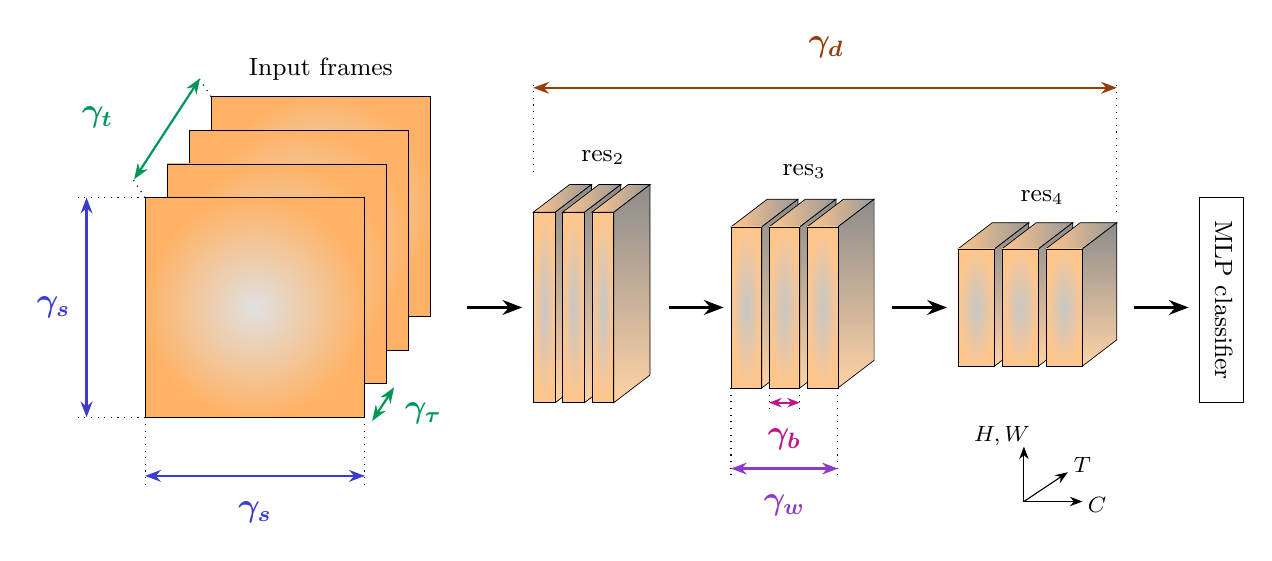
\begin{tikzpicture}[x=0.93cm, y=0.93cm, font=\small]

        % ---------------- input frames ----------------
        \foreach \i in {3,2,1,0}{
            \shadedraw[line width=0.25pt, inner color=black!12, outer color=orange!60]
                (\i*0.30,\i*0.46) rectangle (\i*0.30+3,\i*0.46+3);
        }
        \node at (2.4,4.75) {Input frames};

        % gamma_s : spatial resolution (height and width)
        \draw[dotted] (0,0) -- (-0.95,0);   \draw[dotted] (0,3) -- (-0.95,3);
        \draw[{Stealth[length=2mm]}-{Stealth[length=2mm]}, x3dblue, line width=0.8pt]
            (-0.8,0) -- (-0.8,3);
        \node[font=\large] at (-1.25,1.5) {$\xgs$};
        \draw[dotted] (0,0) -- (0,-0.95);   \draw[dotted] (3,0) -- (3,-0.95);
        \draw[{Stealth[length=2mm]}-{Stealth[length=2mm]}, x3dblue, line width=0.8pt]
            (0,-0.8) -- (3,-0.8);
        \node[font=\large] at (1.5,-1.3) {$\xgs$};

        % gamma_t : temporal duration (stacking direction)
        \draw[dotted] (0,3) -- (-0.2,3.3);  \draw[dotted] (0.9,4.38) -- (0.7,4.68);
        \draw[{Stealth[length=2mm]}-{Stealth[length=2mm]}, x3dgreen, line width=0.8pt]
            (-0.15,3.25) -- (0.75,4.63);
        \node[font=\large] at (-0.65,4.1) {$\xgt$};

        % gamma_tau : frame rate
        \draw[{Stealth[length=2mm]}-{Stealth[length=2mm]}, x3dgreen, line width=0.8pt]
            (3.1,-0.05) -- (3.4,0.41);
        \node[font=\large] at (3.8,0.05) {$\xgtau$};

        % ---------------- stages ----------------
        \draw[-{Stealth[length=2.5mm]}, line width=1.1pt] (4.4,1.5) -- (5.15,1.5);
        \xstage{5.3}{0.2}{0.30}{2.6}{0.9}{0.10}
        \node at (6.25,3.55) {res$_2$};

        \draw[-{Stealth[length=2.5mm]}, line width=1.1pt] (7.15,1.5) -- (7.9,1.5);
        \xstage{8.0}{0.4}{0.42}{2.2}{0.9}{0.10}
        \node at (9,3.35) {res$_3$};

        \draw[-{Stealth[length=2.5mm]}, line width=1.1pt] (10.2,1.5) -- (10.95,1.5);
        \xstage{11.1}{0.7}{0.50}{1.6}{0.85}{0.10}
        \node at (12.25,3.0) {res$_4$};

        \draw[-{Stealth[length=2.5mm]}, line width=1.1pt] (13.5,1.5) -- (14.25,1.5);
        \draw[fill=white] (14.4,0.2) rectangle (15,3);
        \node[rotate=-90] at (14.73,1.6) {MLP classifier};

        % gamma_b : bottleneck width (one slab of res_3)
        \draw[dotted] (8.52,0.4) -- (8.52,0.1);  \draw[dotted] (8.94,0.4) -- (8.94,0.1);
        \draw[{Stealth[length=1.6mm]}-{Stealth[length=1.6mm]}, x3dmagenta, line width=0.8pt]
            (8.52,0.2) -- (8.94,0.2);
        \node[font=\large] at (8.73,-0.3) {$\xgb$};

        % gamma_w : width of the whole res_3 stage
        \draw[dotted] (8.0,0.4) -- (8.0,-0.8);   \draw[dotted] (9.46,0.4) -- (9.46,-0.8);
        \draw[{Stealth[length=2mm]}-{Stealth[length=2mm]}, x3dviolet, line width=0.8pt]
            (8.0,-0.7) -- (9.46,-0.7);
        \node[font=\large] at (8.73,-1.2) {$\xgw$};

        % gamma_d : depth (number of stages)
        \draw[dotted] (5.3,3.35) -- (5.3,4.6);   \draw[dotted] (13.27,2.8) -- (13.27,4.6);
        \draw[{Stealth[length=2mm]}-{Stealth[length=2mm]}, x3dbrown, line width=0.8pt]
            (5.3,4.5) -- (13.27,4.5);
        \node[font=\large] at (9.3,5.05) {$\xgd$};

        % axis legend
        \draw[-{Stealth[length=1.6mm]}] (12.0,-1.15) -- (12.0,-0.4);
        \node[font=\footnotesize] at (11.7,-0.25) {$H,W$};
        \draw[-{Stealth[length=1.6mm]}] (12.0,-1.15) -- (12.6,-0.75);
        \node[font=\footnotesize] at (12.8,-0.65) {$T$};
        \draw[-{Stealth[length=1.6mm]}] (12.0,-1.15) -- (12.8,-1.15);
        \node[font=\footnotesize] at (13.0,-1.2) {$C$};

    \end{tikzpicture}
    \caption{\textbf{X3D} networks progressively expand a 2D network across the following axes: temporal duration $\xgt$, frame rate $\xgtau$, spatial resolution $\xgs$, width $\xgw$, bottleneck width $\xgb$, and depth $\xgd$. Redrawn after \cite{feichtenhofer2020x3d}.}
    \label{fig:x3d_expand}
\end{figure}

Having introduced possible scaling dimensions suggested in the paper, we show two key expansion regimes underpinning their discovery of network architectures.
It is noteworthy that, there are different sizes of \texttt{X3D} depending how many times \texttt{X2D} is progressively scaled using the aforementioned expansion operations.
Remarkably, the computation/accuracy trade–off is controlled by utilising a feature selection method, i.e. forward selection and backward elimination \cite{feat_select}.


\paragraph{Forward expansion.} At each iteration, the algorithm loops through all possibilities by changing a factor in $\Gamma \triangleq \{\xgtau, \xgt, \xgs, \xgw, \xgb, \xgd\}$ and keeping others unchanged. Two important factors driving the choice of scaling dimensions are.
First, the goodness criterion function $J(\Gamma)$, which is chosen to be the accuracy gained by expanding the current model by $\Gamma$, and thus, the higher the better.
Second, computing resources are of paramount importance, and hence, deserved to be considered during the expansion.
Let us denote $C(\Gamma)$ be a complexity criterion function, specifically FLOPs measurement in \cite{feichtenhofer2020x3d}.
Ultimately, each iteration, the algorithm opts out the best balance between accuracy and complexity. Formally, $\Gamma = \operatorname*{\arg\max}\limits_{\mathcal Z, ~C(\mathcal Z) = c} J(\mathcal Z)$, where $\mathcal Z$ are possibilities of varying $\Gamma$ and $c$ is the target complexity budget.

Remarkably, one may notice, there can be at most $2^6$ ways to change, each of which exhausts the computational capacity by varying $c \in \mathbb R$.
Therefore, they rely on the idea of coordinate descent algorithms \cite{Wright2015CoordinateDA} and fixing the expansion rate at $c \approx 2$.
In order to ensure this expansion rate, \cite{feichtenhofer2020x3d} provides details how much each scaling dimension can be expanded coordinate–wise.

\paragraph{Backward contraction.} Simply speaking, this step is introduced to the algorithm to reduce $C(\mathcal Z)$ when its target complexity is surpassed in the prior forward expansion, so that $C(\mathcal Z) < c$ is guaranteed at each iteration.


\subsection{X3D family}

\begin{table}[H]
    \centering
    \renewcommand{\arraystretch}{1.4}
    \setlength{\tabcolsep}{9pt}
    \setlength{\arraycolsep}{10pt}
    \begin{tabular}{c|c|c@{\hspace{7pt}}l}
        \cline{1-3}
        stage & filters & output sizes $T\times S^2$ & \\
        \cline{1-3}\noalign{\vskip1.2pt}\cline{1-3}
        data layer & stride $\xgtau,\ 1^2$ & $1\xgt\times(112\xgs)^2$ & \\
        \cline{1-3}
        conv$_1$ & $1\times3^2,\ 3\times1,\ 24\xgw$ & $1\xgt\times(56\xgs)^2$
            & $\left.\rule[-8pt]{0pt}{16pt}\right\}$ \texttt{blocks[0]} \\
        \cline{1-3}
        res$_2$ & $\resblock{24}{}$ & $1\xgt\times(28\xgs)^2$
            & $\left.\rule[-25pt]{0pt}{50pt}\right\}$ \texttt{blocks[1]} \\
        \cline{1-3}
        res$_3$ & $\resblock{48}{2}$ & $1\xgt\times(14\xgs)^2$
            & $\left.\rule[-25pt]{0pt}{50pt}\right\}$ \texttt{blocks[2]} \\
        \cline{1-3}
        res$_4$ & $\resblock{96}{5}$ & $1\xgt\times(7\xgs)^2$
            & $\left.\rule[-25pt]{0pt}{50pt}\right\}$ \texttt{blocks[3]} \\
        \cline{1-3}
        res$_5$ & $\resblock{192}{3}$ & $1\xgt\times(4\xgs)^2$
            & $\left.\rule[-25pt]{0pt}{50pt}\right\}$ \texttt{blocks[4]} \\
        \cline{1-3}
        conv$_5$ & $1\times1^2,\ 192\xgb\xgw$ & $1\xgt\times(4\xgs)^2$
            & \multirow{4}{*}{$\left.\rule[-34pt]{0pt}{68pt}\right\}$ \texttt{blocks[5]}} \\
        pool$_5$ & $1\xgt\times(4\xgs)^2$ & $1\times1\times1$ & \\
        fc$_1$ & $1\times1^2,\ 2048$ & $1\times1\times1$ & \\
        fc$_2$ & $1\times1^2,\ \#\text{classes}$ & $1\times1\times1$ & \\
        \cline{1-3}
    \end{tabular}
    \caption{\textbf{X3D architecture} \cite{feichtenhofer2020x3d}. The dimensions of kernels are denoted by $\{T\times S^2, C\}$ for temporal, spatial, and channel sizes. Strides are denoted as $\{$temporal stride, spatial stride$^2\}$. This network is expanded using factors $\{\xgtau, \xgt, \xgs, \xgw, \xgb, \xgd\}$ to form \texttt{X3D}. The braces on the right give the corresponding entry of the \texttt{blocks} module list of the \texttt{PyTorchVideo} implementation \cite{fan2021pytorchvideo}, i.e. the stem \texttt{blocks[0]}, the four residual stages \texttt{blocks[1]} to \texttt{blocks[4]}, and the head \texttt{blocks[5]}. The data layer is a sampling step so no trainable parameters required.}
    \label{tab:x3d_arch}
\end{table}

% This grouping is the unit of adaptation used in \textbf{Section \ref{sec:experiment}}, where freezing $k$ blocks means holding \texttt{blocks[0]} to \texttt{blocks[$k-1$]} fixed, so that $k = 0$ trains the whole network and $k = 5$ trains the classifier head alone.
Concretely, \texttt{X3D} is a feature extractor of a video. Conceptually, this can be represented using the following diagram:

\begin{figure}[H]
    \centering
    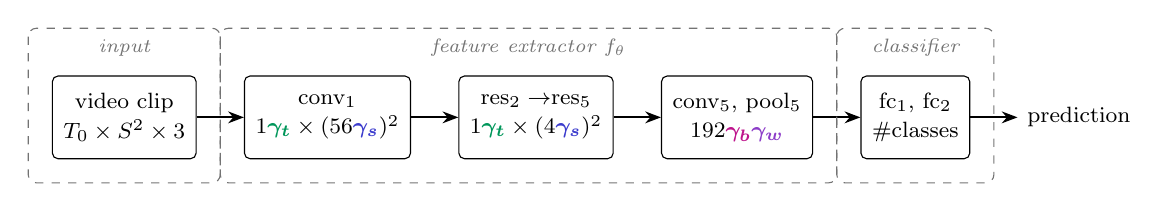
\begin{tikzpicture}[
        font=\footnotesize,
        box/.style={draw, rounded corners=2pt, align=center, minimum height=1.05cm, inner sep=4pt},
        ar/.style={-{Stealth[length=2mm]}, line width=0.7pt}
    ]
        \node[box]                    (in)   {video clip\\[1pt]$T_0\times S^2 \times 3$};
        \node[box, right=6mm of in]   (stem) {conv$_1$\\[1pt]$1\xgt\times(56\xgs)^2$};
        \node[box, right=6mm of stem] (bb)   {res$_2\to$res$_5$\\[1pt]$1\xgt\times(4\xgs)^2$};
        \node[box, right=6mm of bb]   (head) {conv$_5$, pool$_5$\\[1pt]$192\xgb\xgw$};
        \node[box, right=6mm of head] (fc)   {fc$_1$, fc$_2$\\[1pt]$\#$classes};
        \node[right=6mm of fc]        (out)  {prediction};

        \foreach \a/\b in {in/stem, stem/bb, bb/head, head/fc, fc/out}{\draw[ar] (\a) -- (\b);}

        \draw[dashed, rounded corners=3pt, black!55]
            ($(in.north west)+(-3mm,6mm)$) rectangle ($(in.south east)+(3mm,-3mm)$);
        \node[font=\scriptsize\itshape, black!55]
            at ($(in.north)+(0,3.5mm)$) {input};

        \draw[dashed, rounded corners=3pt, black!55]
            ($(stem.north west)+(-3mm,6mm)$) rectangle ($(head.south east)+(3mm,-3mm)$);
        \node[font=\scriptsize\itshape, black!55]
            at ($(stem.north west)!0.5!(head.north east)+(0,3.5mm)$) {feature extractor $f_\theta$};

        \draw[dashed, rounded corners=3pt, black!55]
            ($(fc.north west)+(-3mm,6mm)$) rectangle ($(fc.south east)+(3mm,-3mm)$);
        \node[font=\scriptsize\itshape, black!55] at ($(fc.north)+(0,3.5mm)$) {classifier};
    \end{tikzpicture}
    \caption{\texttt{X3D} as a video feature extractor followed by a linear classifier. The shape below each stage is its output size, following \textbf{Table \ref{tab:x3d_arch}}. In the input stage, $T_0$ is the total frames in the raw video input and $3$ implies each video's frame is in RGB color space.}
    \label{fig:x3d_pipeline}
\end{figure}

The 2D CNN processes the whole image by learning local information stage by stage, untill the final blocks are sufficiently dense,
and hence, a classfier, typically MLP, is used to yield final prediction.
The 3D CNN generalises this concept by considering multiple frames at once, thereby allowing the model to understand the underlying temporal dependence inherently in video data, and keeps other aspects of 2D CNN as is.
Put simply, both 2D and 3D CNNs are simply feature extractors, said differently, it learns to transform raw data into numerically meaningful vectors.

Due to limited computing resources, we shall skip the expansion of \texttt{X2D} to \texttt{X3D}, and directly leverage different variants of \texttt{X3D} models, supported by \texttt{PyTorchVideo}, to conduct the experiments in the upcoming sections.



%=========================================================


%=========================================================
\newpage
\section{Experiments}
\label{sec:experiment}

\subsection{Datasets}
In short, their motivation for creation of the \texttt{AUTSL} dataset is to replicate the real–world scenarios when using sign languages.
The dataset contains frequently used vocabularies in spoken language, and keep the dataset balanced in terms of motion characteristics and time taken to complete a word.
\textbf{Table \ref{tab:AUTSL_description}} below shows an overview of the dataset.

\begin{table}[H]
\centering\small
\begin{tabular}{@{}c c@{}}
\toprule
\textbf{Property} & \textbf{Description}  \\
\midrule
Number of signs & $226$  \\
Number of signers & $43$ \\
Total samples & $38,336$ \\
Number of different backgrounds &  $20$ \\
Mean sample per sign & $169.6$ \\
Modalities & RGB, depth, skeleton \\
RGB and depth resolution & $512 \times 512$ \\
FPS & 30 \\
\bottomrule
\end{tabular}
\caption{Statistics of AUTSL dataset \cite{sincan2020autsl}.}
\label{tab:AUTSL_description}
\end{table}

Regarding challenges, the videos span a wide variety of static and dynamic backgrounds, the latter containing objects moving behind the signer.
The authors further selected signs that are very similar in motion and separated only by subtle gestures, included compound signs built from simpler ones, and recruited signers of differing backgrounds, so that personal signing style varies across the dataset.


In this experiment, we leverage the available \texttt{AUTSL} dataset given in Kaggle, accessible via \href{https://www.kaggle.com/datasets/sttaseen/autsl}{this link}.
This dataset only comprises of RGB-colored videos, for a comprehensive dataset of \texttt{AUTSL}, including different video formats of the same data, refer to \href{https://cvml.ankara.edu.tr/datasets/}{this link}.
Therefore, by utilisation of Kaggle dataset, we limit ourselves to benchmark \texttt{X3D} performance on RGB–colored videos. Lastly, the downloaded data was already partitioned, and thus, we shall not split the dataset by our own.

\begin{table}[H]
\centering\small
\begin{tabular}{@{}c c c@{}}
\toprule
\textbf{Set} & \textbf{Number of samples} & \textbf{Percentage}  \\
\midrule
Train & $28,142$ & $77.5\%$ \\
Validation & $4,418$ & $12.2\%$ \\
Test & $3,742$ & $10.3\%$ \\
\midrule
Total & $36,302$ & 100\% \\
\bottomrule
\end{tabular}
\caption{Number of samples inspected directly from the dataset.}
\label{tab:AUTSL_samples}
\end{table}

Apparently, \textbf{Table \ref{tab:AUTSL_description}} and \textbf{Table \ref{tab:AUTSL_samples}} differ in the total number of samples, suggesting a data shift between the Kaggle release and the original.
We therefore re–inspect the dataset from its filenames in \textbf{Figure \ref{fig:data-inspect-1}} and \textbf{Figure \ref{fig:data-inspect-2}}, which still count every clip.
Of these, $11$ are truncated and cannot be decoded, i.e. $10$ in train and $1$ in test, and are excluded from both training and testing, leaving the $28{,}132$ and $3{,}741$ clips actually used.

\begin{figure}[H]
    \centering
    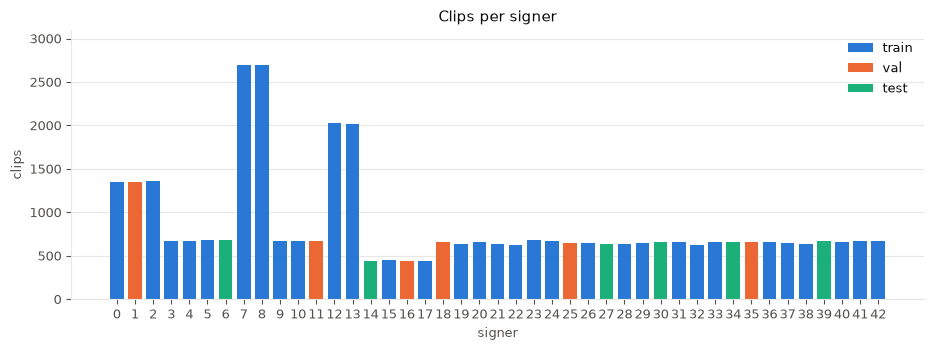
\includegraphics[width=1\textwidth]{figures/data_inspect_1.png}
    \caption{Inspection of number of clips produced by each signer.}
    \label{fig:data-inspect-1}
\end{figure}

\begin{figure}[H]
    \centering
    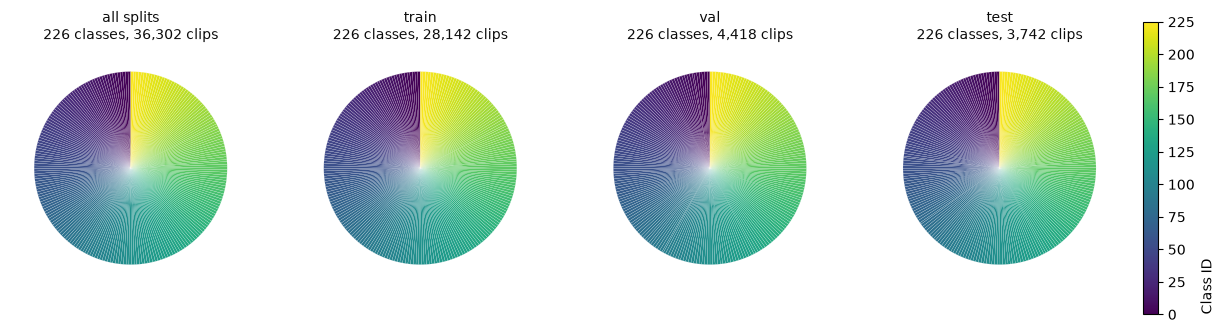
\includegraphics[width=\textwidth]{figures/data_inspect_2.png}
    \caption{Distribution of sign classes across the dataset splits. Every split covers all $226$ classes.
    \textbf{All splits:} $36{,}302$ clips, with min $121$, median $162$, mean $160.6$ and max $164$ clips per class.
    \textbf{train:} $28{,}142$ clips (min $90$, median $126$, mean $124.5$, max $127$)
    \textbf{validation:} $4{,}418$ clips (min $12$, median $20$, mean $19.5$, max $20$)
    \textbf{test:} $3{,}742$ clips (min $10$, median $17$, mean $16.6$, max $17$).}
    \label{fig:data-inspect-2}
\end{figure}

\paragraph{Dataset building.} According to the models' sizes in \href{https://github.com/facebookresearch/pytorchvideo/blob/f3142bb05cdb56af0704ab6f0adfb0c7bbafe4a0/pytorchvideo/models/x3d.py#L539}{this code}, we adopt the clip geometry summarised in \textbf{Table \ref{tab:model_sizes}}.
\begin{table}[H]
    \centering\small
    \begin{tabular}{@{}c c c@{}}
    \toprule
    \textbf{Model size} & \texttt{num\_frames} & \texttt{crop\_size}  \\
    \midrule
    \texttt{X3D\_XS} & $4$ & $160$  \\
    \texttt{X3D\_S} & $13$ & $160$  \\
    \texttt{X3D\_M} & $16$ & $224$  \\
    \bottomrule
    \end{tabular}
    \caption{Number of frames and crop size for each video.}
    \label{tab:model_sizes}
\end{table}
\texttt{AUTSL} dataset must be built with the matching \texttt{num\_frames} and \texttt{crop\_size}, otherwise the weights load but the model sees inputs it was never trained for.

\subsection{Implementation details}
\label{sec:implementation}
% Describe the experimental environment


In this experiment, we do not benchmark the model against other methods. Alternatively, we benchmark different fine-tuning approaches of different models' sizes.

In the original codebase, \texttt{X3D} was pretrained on \texttt{Kinetics--400} dataset \cite{kay2017kinetics}, and thus the final \texttt{softmax} layer does not match the number of classes in \texttt{AUTSL} dataset.
Therefore, we replace the final linear projection layer, to reduce the number of classes.
Formally, let $g(\mathbf x)$ is the final fully connected layer of pretrained \texttt{X3D}, given by:
\begin{align}
    g: \mathbb R^{k} \mapsto \mathbb R^{400}
\end{align}
We shall replace it by:
\begin{align}
    g: \mathbb R^k \mapsto \mathbb R^{226}
\end{align}

The remaining settings are as follows.
\begin{itemize}[topsep=2pt, itemsep=2pt]
    \item \textbf{Data.} The \texttt{AUTSL} train split, i.e. $28{,}142 - 10 = 28{,}132$ clips over $226$ classes, unless a subset is configured.
    \item \textbf{Preprocessing.} Uniform temporal subsampling to the variant's clip length, resizing to its crop size, random horizontal flip, scaling to $[0,1]$ and per--channel normalisation with mean $0.45$ and standard deviation $0.225$.
    \item \textbf{Initialisation.} \texttt{Kinetics--400} weights for the backbone, and a freshly initialised linear head.
    \item \textbf{Optimisation.} Cross--entropy loss with \texttt{Adam}. About fine–tuning different components, frozen blocks are excluded from the optimiser and held in evaluation mode, so that their \texttt{BatchNorm} running statistics do not drift.
    \item \textbf{Hyperparameters.} Epochs = 100, batch size = 16 and learning rate = $10^{-4}$.
    \item \textbf{Hardware.} AMD EPYC 7402P (24 cores - 48 threads), 256 GB DDR4 RAM and 4x NVIDIA A100 (40GB HBM2 each).
\end{itemize}




\subsection{Evaluation metrics}
\label{sec:metrics}

Since \texttt{X3D} is designed around an accuracy–complexity trade-off rather than accuracy alone \cite{feichtenhofer2020x3d}, we report metrics along two axes, i.e. how well a model recognises signs, and how expensive it is to store and to evaluate.
% Reporting only the former would conceal exactly the property that motivates this family of networks \cite{tan2019efficientnet, MoViNets}.

\paragraph{Top–$k$ accuracy.}
Let the test split be $\mathcal D = \{(\mathbf V_i, y_i)\}_{i=1}^{N}$, where $\mathbf V_i$ is a clip and $y_i \in \{1, \ldots, C\}$ is its sign label, $C = 226$ being the number of classes.
For each clip the network, i.e. the final \texttt{softmax} layer, produces a score vector $\mathbf z_i = (z_{i1}, \ldots, z_{iC}) \in \mathbb R^C$, and we write $\mathcal R_k(\mathbf V_i) \subseteq \{1, \ldots, C\}$ to denote the subset of $k \le C$ classes receiving the largest scores.
The top–$k$ accuracy:
\begin{align}
    \text{top--}k = \frac{1}{N} \sum_{i=1}^{N} \mathbf 1 \left\{ y_i \in \mathcal R_k(\mathbf V_i) \right\},
\end{align}
where $\mathbf 1\{\cdot\}$ denotes the indicator function.
% As the \texttt{softmax} map is strictly increasing, it preserves the ordering of $\mathbf z_i$, and hence $\mathcal R_k$ may equivalently be taken over logits.

We evaluate $k \in \{1, 3, 5\}$, and note that
$\mathcal R_1 \subseteq \mathcal R_3 \subseteq \mathcal R_5 \Rightarrow \text{Top--}1 \le \text{Top--}3 \le \text{Top--}5$.
Top–1 is the strict accuracy, i.e. the fraction of clips whose most probable class is correct, and is the quantity of practical interest for a recognition system.
Top–5 is the conventional companion metric on \texttt{Kinetics–400} \cite{kay2017kinetics} and \texttt{ImageNet} \cite{Russakovsky2015}.
Top–3 is included to give balance between strict metric top–1 and easy metric top–5.
The margin between Top–1 and Top–3 therefore diagnoses the nature of the residual errors, i.e. a small margin indicates genuine failures, whereas a large one indicates near misses within a small group of mutually confusable signs.

\paragraph{Total and trainable parameters.}
Let $\theta$ be the full set of parameters of a model and $\theta_{\text{tr}} \subseteq \theta$ the subset left unfrozen during training.
We report the cardinalities $|\theta|$ and $|\theta_{\text{tr}}|$.
Because our experiments compare fine–tuning strategies rather than competing architectures, this pair separates two costs that a single count would conflate.
$|\theta|$ governs the memory required to store and deploy the network, whereas $|\theta_{\text{tr}}|$ governs the gradients and optimiser state held during training, and thus the cost of adaptation.
% A frozen backbone with a retrained head leaves $|\theta|$ essentially unchanged while making $\rho \ll 1$; full fine--tuning gives $\rho = 1$.

\paragraph{GFLOPs.}
We quantify inference cost by the number of floating–point operations required for one forward pass, expressed in units of $10^9$.
Following the convention adopted in \cite{feichtenhofer2020x3d, tan2019efficientnet}, we count multiply--adds and quote the cost of a \textit{single} clip.
% a test--time protocol that averages predictions over several temporal clips and spatial crops multiplies this figure by the number of views.
% Two remarks are in order.
% First, unlike the image setting, the cost of a video network depends on the shape $T \times S^2$ of the sampled clip, so this shape must be fixed before the figures of different variants may be compared.
Importantly, GFLOPs is an analytic quantity, independent of hardware, and is therefore a fair proxy for arithmetic effort but not for wall--clock latency.
% as \cite{MoViNets} observes, peak memory consumption may dominate the practical cost of a video model on constrained devices.





\subsection{Main results}
\label{sec:results}

% Figures are written to <root>/figures by src/main.py and src/evaluate.py.
% Copy the ones cited below into report/figures/ before compiling, since
% \includegraphics resolves relative to this directory.
% Numbers marked in red are filled from results/metrics.csv once the runs finish.

% \pending draws the figure once a run has produced it, and a labelled box
% until then, so the report compiles at every stage of the experiments.
\providecommand{\pending}[2][\textwidth]{%
    \IfFileExists{#2}{\includegraphics[width=#1]{#2}}{%
        \fbox{\parbox[c][3cm][c]{\dimexpr#1-2\fboxsep-2\fboxrule\relax}{%
            \centering\footnotesize\texttt{\detokenize{#2}}\\[4pt]
            \normalfont\textcolor{red}{awaiting the run}}}%
    }%
}

% Due to the challenges inherent in the dataset, we do not expect \texttt{X3D} to perform comparably to purpose–built sign language models, but rather to reach an acceptable accuracy while retaining an inference cost small enough for edge deployment.
% Following \textbf{Sec. \ref{sec:introduction}}, we are further interested in how far fine–tuning depth affects that trade–off.

\subsubsection{Learning behaviour on train/validation sets}

We train every combination of the three variants \texttt{X3D\_XS}, \texttt{X3D\_S} and \texttt{X3D\_M} with $0$ to $5$ of the six blocks held frozen.
\textbf{Figure \ref{fig:curves}} shows the two extremes of this sweep, and \textbf{Table \ref{tab:val_sweep}} collects the best validation top--1 of every run.

\begin{figure}[H]
    \centering
    \begin{subfigure}[b]{0.49\textwidth}
        \pending{figures/learning/x3d_xs_freeze5.png}
        \caption{\texttt{X3D\_XS}, head only.}
    \end{subfigure}
    \hfill
    \begin{subfigure}[b]{0.49\textwidth}
        \pending{figures/learning/x3d_xs_freeze0.png}
        \caption{\texttt{X3D\_XS}, full fine--tune.}
    \end{subfigure}

    \vspace{0.4em}

    \begin{subfigure}[b]{0.49\textwidth}
        \pending{figures/learning/x3d_s_freeze5.png}
        \caption{\texttt{X3D\_S}, head only.}
    \end{subfigure}
    \hfill
    \begin{subfigure}[b]{0.49\textwidth}
        \pending{figures/learning/x3d_s_freeze0.png}
        \caption{\texttt{X3D\_S}, full fine--tune.}
    \end{subfigure}

    \vspace{0.4em}

    \begin{subfigure}[b]{0.49\textwidth}
        \pending{figures/learning/x3d_m_freeze5.png}
        \caption{\texttt{X3D\_M}, head only.}
    \end{subfigure}
    \hfill
    \begin{subfigure}[b]{0.49\textwidth}
        \pending{figures/learning/x3d_m_freeze0.png}
        \caption{\texttt{X3D\_M}, full fine--tune.}
    \end{subfigure}
    \caption{Per--epoch cross--entropy loss and top--1 accuracy on the train and validation splits, for the two extreme fine--tuning depths of each variant. Freezing five blocks leaves only the classifier trainable, whereas freezing none updates the whole network.}
    \label{fig:curves}
\end{figure}

\begin{table}[H]
\centering\small
\begin{tabular}{@{}c cc cc cc@{}}
\toprule
\textbf{Frozen} & \multicolumn{2}{c}{\texttt{X3D\_XS}} & \multicolumn{2}{c}{\texttt{X3D\_S}} & \multicolumn{2}{c}{\texttt{X3D\_M}} \\
\cmidrule(lr){2-3}\cmidrule(lr){4-5}\cmidrule(lr){6-7}
\textbf{blocks} & train & val & train & val & train & val \\
\midrule
$0$ & $95.4$ & $63.9$ & $98.3$ & $\mathbf{81.5}$ & $98.4$ & $85.4$ \\
$1$ & $95.4$ & $\mathbf{64.7}$ & $98.4$ & $80.4$ & $98.3$ & $85.5$ \\
$2$ & $95.5$ & $64.2$ & $98.4$ & $81.0$ & $98.9$ & $\mathbf{86.1}$ \\
$3$ & $93.7$ & $58.7$ & $98.5$ & $75.8$ & $98.7$ & $83.4$ \\
$4$ & $92.4$ & $49.2$ & $97.7$ & $71.1$ & $97.8$ & $77.1$ \\
$5$ & $48.0$ & $19.9$ & $64.3$ & $36.5$ & $69.8$ & $38.5$ \\
\bottomrule
\end{tabular}
\caption{Top--1 accuracy (\%) on the train and validation splits, for each variant and freezing depth. The variants differ only in the clip they sample, i.e. \texttt{X3D\_XS} takes $4$ frames at $160^2$, \texttt{X3D\_S} $13$ frames at $160^2$ and \texttt{X3D\_M} $16$ frames at $224^2$. The best validation entry per variant is bolded.}
\label{tab:val_sweep}
\end{table}

\paragraph{Underfitting.} Training the classifier head only amount to underfitting, evidently $48.0\%$, $64.3\%$ and $69.8\%$ accuracy for \texttt{X3D\_XS}, \texttt{X3D\_S} and \texttt{X3D\_M}, respectively.
This is indicative of the \texttt{Kinetics–400} pretrained weights may not contribute vastly to models' performance on \texttt{AUTSL}, and mostly rely on the learning capacity of the classifier block.

\paragraph{Pretrained weights may not help.} Looking at learning curves in \textbf{Figure \ref{fig:curves}}, at the first few epochs, they accuracy is extremely low.
Semantically, this is true, since \texttt{Kinetics–400} and \texttt{AUTSL} are constructed for two completely different tasks. Nonetheless, we cannot strongly claim that this does not help, since the pretrained weights may yield a relatively good initial starting point to optimise the models, in terms of local optimality and convergence speed.
Further ablation studies must be conducted to compare between train–from–scratch vs. train–from–pretrained.

\paragraph{Overfitting.} Interestingly, enabling more blocks in the backbone model trainable flips the situation. It immediately overfits to the training data for the first block adjacent to the classifier head, evidently by the huge gap between train and validation accuracy.
Nevertheless, the gap is converging as we allows more parameters learnable, and astonishingly, such train–validation gap is narrower in \texttt{X3D\_M} than in \texttt{X3D\_XS}.

\paragraph{Clip sampling outweighs adaptation depth.} The ordering $\texttt{X3D\_M} > \texttt{X3D\_S} > \texttt{X3D\_XS}$ holds at every freezing depth, and the margin is large.
More specifically, on validation accuracy, \texttt{X3D\_M} with three blocks frozen ($83.4\%$), fully fine–tuned ``best'' \texttt{X3D\_S} ($81.5\%$), and one block frozen ``best'' \texttt{X3D\_XS} ($64.7\%$).
From \textbf{Table \ref{tab:main_results}}, three variants differ only in the clip drawn from each video and the cropping size each frame.
Therefore, the gain is attribute to temporal and spatial sampling rather than to capacity, and it is traded off with GFLOPs.

\paragraph{Recommendation.} From the above–mentioned results and analysis, we shall pick \texttt{X3D\_M} with 2 frozen blocks as our ``best'' model, due to its performance competency and good trade–off with trainable parameters.

\subsubsection{Final evaluation on test set}

\begin{table}[H]
\centering\small
\begin{tabular}{@{}l c c c c c c c@{}}
\toprule
\textbf{Model} & \textbf{Frozen} & \textbf{Top--1} & \textbf{Top--3} & \textbf{Top--5} & \textbf{Params} & \textbf{Trainable} & \textbf{GFLOPs} \\
 & & (\%) & (\%) & (\%) & (M) & (M) & \\
\midrule
\texttt{X3D\_XS} & $0$ & $54.08$ & $72.36$ & $78.40$ & $3.438$ & $3.438$ & $0.63$ \\
\texttt{X3D\_XS} & $1$ & $\mathbf{56.91}$ & $74.58$ & $80.78$ & $3.438$ & $3.437$ & $0.63$ \\
\texttt{X3D\_XS} & $2$ & $53.49$ & $73.08$ & $79.76$ & $3.438$ & $3.422$ & $0.63$ \\
\texttt{X3D\_XS} & $3$ & $49.67$ & $69.31$ & $76.90$ & $3.438$ & $3.348$ & $0.63$ \\
\texttt{X3D\_XS} & $4$ & $38.89$ & $58.49$ & $66.61$ & $3.438$ & $2.779$ & $0.63$ \\
\texttt{X3D\_XS} & $5$ & $14.68$ & $26.01$ & $31.36$ & $3.438$ & $1.432$ & $0.63$ \\
\midrule
\texttt{X3D\_S} & $0$ & $75.67$ & $89.74$ & $93.42$ & $3.438$ & $3.438$ & $2.03$ \\
\texttt{X3D\_S} & $1$ & $\mathbf{76.56}$ & $89.76$ & $93.26$ & $3.438$ & $3.437$ & $2.03$ \\
\texttt{X3D\_S} & $2$ & $75.67$ & $89.60$ & $93.50$ & $3.438$ & $3.422$ & $2.03$ \\
\texttt{X3D\_S} & $3$ & $69.85$ & $85.89$ & $90.35$ & $3.438$ & $3.348$ & $2.03$ \\
\texttt{X3D\_S} & $4$ & $63.46$ & $81.05$ & $86.93$ & $3.438$ & $2.779$ & $2.03$ \\
\texttt{X3D\_S} & $5$ & $29.35$ & $43.89$ & $50.12$ & $3.438$ & $1.432$ & $2.03$ \\
\midrule
\texttt{X3D\_M} & $0$ & $\mathbf{82.38}$ & $93.50$ & $95.94$ & $3.438$ & $3.438$ & $4.90$ \\
\texttt{X3D\_M} & $1$ & $80.83$ & $92.70$ & $95.64$ & $3.438$ & $3.437$ & $4.90$ \\
\texttt{X3D\_M} & $2$ & $82.28$ & $94.49$ & $96.52$ & $3.438$ & $3.422$ & $4.90$ \\
\texttt{X3D\_M} & $3$ & $77.17$ & $90.56$ & $94.04$ & $3.438$ & $3.348$ & $4.90$ \\
\texttt{X3D\_M} & $4$ & $73.62$ & $89.20$ & $93.40$ & $3.438$ & $2.779$ & $4.90$ \\
\texttt{X3D\_M} & $5$ & $34.86$ & $50.98$ & $57.31$ & $3.438$ & $1.432$ & $4.90$ \\
\bottomrule
\end{tabular}
\caption{Performance on the \texttt{AUTSL} test split ($3{,}741$ clips evaluated over $226$ classes). The best top–1 per variant is bolded.}
\label{tab:main_results}
\end{table}

\paragraph{Freezing depth.} Training the whole network rather than the head alone adds $39.4$, $46.3$ and $47.5$ top--1 points for \texttt{X3D\_XS}, \texttt{X3D\_S} and \texttt{X3D\_M}, at $2.4\times$ the trainable parameters.
Interestingly, by unfreezing only one block adjacent to the head block, i.e. \texttt{res}$_5$, lifts \texttt{X3D\_M} from $34.86\%$ to $73.62\%$ for $1.35$M extra trainable parameters, likewise for \texttt{X3D\_XS} and \texttt{X3D\_S}.
Thereafter, unfreezing other blocks gain more accuracy, though not a big jump as before.

\paragraph{Model size.} Moving from \texttt{X3D\_XS} to \texttt{X3D\_S} costs $3.2\times$ the GFLOPs and returns $19.7$ top--1 points; the further step to \texttt{X3D\_M} costs $2.4\times$ again for only $5.8$.
The longer clip is therefore not wasted on isolated signs, but its value saturates.

\paragraph{Error type.} The top--1 to top--3 margin is widest for \texttt{X3D\_XS} and narrowest for \texttt{X3D\_M}.
We shall claim, though insignificantly, that the small variant's errors are largely near misses among confusable signs, whereas the residual errors of \texttt{X3D\_M} are more often outright failures.

\subsubsection{Generalising to our data}

We separate this section from the testing above, since the test split still shares underlying patterns with the train split, e.g. signer identity, background and experimental bias.
To build the dataset we watched the public clips, replicated their motions and annotated with the same numeric \texttt{id}, as the model learnt indexed rather than text--based classes.
Also, it poses more challenges, as we cannot mimic the mouth movements that some signs involve, our lighting is poor and introduces scattering, and \texttt{AUTSL} records the full body whereas we recorded only the upper half.

\paragraph{Setup.} We recorded ten clips on a laptop camera at $1620\times1080$, each imitating one \texttt{AUTSL} sign and named after the test clip whose label it borrows.
In other words, the footage itself is our own and only the labelling convention is shared.
They were converted to \texttt{mp4} and passed through the pipeline of \textbf{Sec. \ref{sec:implementation}}. We run the inference on this hand–crafted data using CPU on MacBook M3 Pro.

\begin{table}[H]
\centering\small
\begin{tabular}{@{}c c c c c@{}}
\toprule
\textbf{Clip} & \textbf{True class} & \textbf{Predicted (top–1)} & \textbf{Confidence} & \textbf{Inference time (s)} \\
\midrule
$0$ & $161$ & $161$ & $1.000$ & 0.369 \\
$1$ & $77$  & $77$  & $0.667$ & 0.331\\
$2$ & $22$  & $18$  & $0.974$ & 0.343\\
$3$ & $157$ & $213$ & $0.860$ & 0.310\\
$4$ & $112$ & $32$  & $0.680$ & 0.328\\
$5$ & $128$ & $54$  & $0.703$ & 0.313\\
$6$ & $14$  & $14$  & $1.000$ & 0.316\\
$7$ & $5$   & $5$   & $1.000$ & 0.340\\
$8$ & $23$  & $23$  & $0.987$ & 0.332\\
$9$ & $155$ & $155$ & $0.999$ & 0.404\\
\bottomrule
\end{tabular}
\caption{Predictions of \texttt{X3D\_M} with two frozen blocks on ten self--recorded clips. Confidence is the \texttt{softmax} probability of the predicted class.}
\label{tab:custom}
\end{table}

\paragraph{Accuracy.} As collected in \textbf{Table \ref{tab:custom}}, the model recognises six of the ten clips, i.e. $60\%$ top--1, $60\%$ top--3 and $70\%$ top--5, yet incomparable with the test results in \textbf{Table \ref{tab:main_results}} due to insufficient samples.

\paragraph{Confidence.} The wrong predictions are as confident as the right ones, i.e. $0.68$ to $0.97$ against $0.67$ to $1.00$.
Softmax confidence therefore offers no usable signal for rejecting an out--of--distribution clip.

\paragraph{Latency.} Inference took $0.310$ to $0.404$ seconds per clip, $0.339$ on average, on a CPU alone.
It suggests the model is deployable for real–time inference.

%=========================================================


%=========================================================
\newpage
\section{Conclusion and discussion}
\label{sec:conclusion}

\paragraph{Conclusion.}
This report summarised \texttt{X3D} \cite{feichtenhofer2020x3d}, the family of video networks obtained by expanding a small 2D architecture one axis at a time, and examined how its \texttt{PyTorchVideo} implementation \cite{fan2021pytorchvideo} transfers to isolated sign language recognition on \texttt{AUTSL} \cite{sincan2020autsl}.
Our best configuration, \texttt{X3D\_M} with two frozen blocks, reaches $82.28\%$ top--1, $94.49\%$ top--3 and $96.52\%$ top--5 on the \texttt{AUTSL} test split, at $4.90$ GFLOPs per clip and $3.42$M trainable parameters.
On the first question, full fine--tuning is worth between $39.4$ and $47.5$ top--1 points over a retrained head, but the gain is unevenly distributed: unfreezing one further block recovers most of it, and freezing the first one or two blocks costs nothing.
On the second, the larger variant repays its cost only in part.
The step from \texttt{X3D\_XS} to \texttt{X3D\_S} returns $19.7$ points for $3.2\times$ the GFLOPs, whereas the step to \texttt{X3D\_M} returns $5.8$ for a further $2.4\times$.
Since all three variants share one parameter count, this is the price of sampling a longer clip rather than of a larger model.

\paragraph{Limitations.}
Each configuration was trained once, so differences of one or two points cannot be separated from seed variance.
Only the RGB modality was used, leaving the depth and skeleton streams of \texttt{AUTSL} unexploited, and GFLOPs measures arithmetic rather than latency on an actual edge device.
Another limitation is, the model can only predicts 226 Turkish isolated signs, any thus, fails to predict out–of–distribution data.

\paragraph{Future work.} \texttt{PyTorchVideo}'s \texttt{X3D} is faster than the original implementation \cite{feichtenhofer2020x3d, pyslowfast}, yet still short of what edge deployment demands.
\texttt{PyTorchVideo} also supports \texttt{EfficientX3D} for that purpose, but only \texttt{X3D\_XS} and \texttt{X3D\_S} carry \texttt{Kinetics–400} weights, \href{https://github.com/facebookresearch/pytorchvideo/blob/f3142bb05cdb56af0704ab6f0adfb0c7bbafe4a0/pytorchvideo/models/hub/efficient_x3d_mobile_cpu.py}{see here}.
Since fine--tuning outperforms training from scratch on small datasets \cite{LI2020103853, 7426826}, as applied to sign language recognition in \cite{10627077, töngi2021applicationtransferlearningsign, shuchang2022surveyhumanactionrecognition, han2022efficient}, we leave \texttt{EfficientX3D} to future work for want of pretrained weights.

%=========================================================


\newpage
\bibliographystyle{splncs04} % or another style like plain, apa, etc.
\bibliography{literature}
% \nocite{*}

%=========================================================
% \appendix
% \newpage
% \section*{Appendices}
% \addcontentsline{toc}{section}{Appendices}

% \section{Notations and Terminology}
% {\renewcommand{\arraystretch}{1.3}
% \section*{Acronyms}
% \begin{tabularx}{\textwidth}{lX}
% \hline
% \textbf{Acronyms} & \textbf{Meaning} \\
% \hline
% DE & Differential Equation \\
% ODE & Ordinary Differential Equation \\
% PDE & Partial Differential Equation \\
% IVP & Initial Value Problem \\
% BVP & Boundary Value Problem \\
% PC & Piecewise Continuous \\
% w.r.t & with respect to \\
% i.e. & that is \\
% e.g. & example \\
% iff & if and only if \\
% JCF & Jordan Canonical Form\\
% IBP & Integration By Parts\\
% FT & Fourier Transform\\
% DFT & Discrete Fourier Transform\\
% FFT & Fast Fourier Transform\\
% \hline
% \end{tabularx}}

% {\renewcommand{\arraystretch}{1.7}
% \section*{Notation}

% \begin{tabularx}{\textwidth}{lX}
% \hline
% \textbf{Symbol} & \textbf{Meaning} \\
% \hline
% $\mathbb{R}$ & Set of real numbers \\
% $\mathbb{C}$ & Set of complex numbers \\
% $\mathbb Z_{\ge 0}$ & Set of non–negative integers \\
% $\mathbf x$ & vectors (in general) \\
% $i = \overline{a, b}$ & $i = a, a+1, \ldots, b$ \\
% $F(\mathbf x, f, \nabla f, \nabla^2 f, \ldots)$ & a set of functions that are added together \\
% $f^{(n)} \equiv \dfrac{d^nf}{dx^n}$ & The $n^{th}$ derivative of $f$ \\[1em]
% $\dfrac{\partial f}{\partial x} \equiv f_x$ & The $1^{st}$–order partial derivative of $f$ w.r.t independent variable $x$\\[1em]
% $\nabla f$ & The ($1^{st}$–order) gradient of $f$ \\
% $D^nf \equiv \nabla^n f$ & The $n^{th}$–order gradient of $f$ \\
% $D^\alpha f$ & The multi–index $\alpha$ of $f$\\
% $H(f)(\mathbf x)$ & The Hessian Matrix of $f$ \\
% $D_{\mathbf u}f(\mathbf x)$ & The directional derivative of $f$ in the direction of $\mathbf u$\\
% $J\mathbf f$ & The Jacobi matrix of $\mathbf f$\\
% $\lambda_i$ & the $i^{th}$ eigenvalue \\
% $\overrightarrow{\lambda_{ij}}$ & the $j^{th}$ (generalized) eigenvector of the $i^{th}$ eigenvalue \\
% $\mathscr O(\cdot)$ & the time complexity of $(\cdot)$ \\
% $V_n$ & the Vandermonde matrix \\
% \hline
% \end{tabularx}}


\end{document}
